\documentclass[12pt,a4paper]{article}  % Document class
\usepackage[utf8]{inputenc}             % UTF-8 encoding
\usepackage{amsmath, amssymb}           % Math packages
\usepackage{graphicx}                    % Include images
\usepackage{geometry}                    % Page margins
\usepackage{hyperref}   
\usepackage{placeins}                 % Hyperlinks
\geometry{margin=1in}                    % 1-inch margins

\title{State of the Art: Glucose Measurement Techniques}
\author{Ahmed Omrani}
\date{\today}

\begin{document}

\maketitle

\tableofcontents
\newpage

\section{Laboratory Plasma Glucose Measurement (Gold Standard)}

\subsection{Introduction}
Laboratory plasma glucose measurement is considered the \textbf{clinical reference method} for glucose determination. It is essential for the diagnosis of diabetes mellitus, patient monitoring, and calibration of other glucose measurement devices such as SMBG (Self-Monitoring of Blood Glucose) and CGM (Continuous Glucose Monitoring) systems \cite{Sacks2011}. This method relies on \textbf{venous plasma} using enzymatic assays, primarily the \textbf{hexokinase} or \textbf{glucose oxidase} methods.

\subsection{Historical and Regulatory Context}
The hexokinase method was first introduced in the 1960s and gradually became the clinical reference due to its superior specificity compared to older chemical reduction methods (e.g., Somogyi-Nelson) \cite{Hagvik2007}. Regulatory bodies such as the \textbf{FDA} and \textbf{ISO 15197:2013} recommend using reference laboratory methods for validating SMBG and CGM devices \cite{CataChem2020}. These methods are traceable to NIST standard reference materials (SRM 917) and form the backbone for device calibration and clinical trials.

\subsection{Analytical Principles}

\subsubsection{Hexokinase Method}
\FloatBarrier
\begin{figure}[h!]
\centering
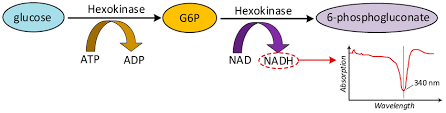
\includegraphics[width=0.8\textwidth]{hexokinase.png} % <-- your file name here
\caption{Workflow for Laboratory Plasma Glucose Measurement using Hexokinase method.}
\label{fig:hexokinase}
\end{figure}
\FloatBarrier
The hexokinase method is the most widely used due to its \textbf{high specificity and precision}. The method involves two main reactions:

\begin{align}
\text{Glucose} + \text{ATP} &\xrightarrow{\text{Hexokinase}} \text{Glucose-6-Phosphate (G6P)} + \text{ADP} \\
\text{G6P} + \text{NAD(P)}^+ &\xrightarrow{\text{G6PD}} 6\text{-Phosphogluconate} + \text{NAD(P)H}
\end{align}

The formation of NAD(P)H is \textbf{directly proportional to glucose concentration} and can be measured spectrophotometrically at 340 nm \cite{StatPearls2025}.

\subsubsection{Glucose Oxidase Method}
The glucose oxidase method catalyzes the reaction:

\[
\text{Glucose} + \text{O}_2 \xrightarrow{\text{Glucose Oxidase}} \text{Gluconolactone} + \text{H}_2\text{O}_2
\]

The produced hydrogen peroxide (\(H_2O_2\)) is then quantified colorimetrically. This method is slightly less specific than hexokinase and can be affected by oxygen levels \cite{Sacks2011}.

\subsection{Analytical Comparison}
\begin{table}[h!]
\centering
\caption{Comparison of Hexokinase and Glucose Oxidase Methods for Plasma Glucose Measurement}
\begin{tabular}{l c c}
\hline
\textbf{Parameter} & \textbf{Hexokinase} & \textbf{Glucose Oxidase} \\
\hline
Specificity & Very high & Moderate \\
Precision (CV) & $\leq 2.5\%$ & 3--5\% \\
Linear range & 0--600 mg/dL & 5--500 mg/dL \\
Sample volume & 0.5--2 mL & 0.5--2 mL \\
Interference & Minimal & Oxygen, uric acid, ascorbate \\
Measurement time & 5--20 min & 5--25 min \\
Reference traceability & ID-MS & No standardized reference \\
\hline
\end{tabular}
\label{tab:method_comparison}
\end{table}
\noindent
\textbf{Table Description:} This table summarizes the main analytical parameters of the two most common laboratory plasma glucose measurement methods. It highlights the \textbf{high specificity and precision} of the hexokinase method versus the glucose oxidase method, which is more susceptible to interference from oxygen and other reducing agents. Linear range, sample volume, measurement time, and reference traceability are also compared to guide method selection in clinical laboratories.
\subsection{Sample Handling and Workflow}
\FloatBarrier
\begin{itemize}
    \item \textbf{Sample type:} Venous blood collected in sodium fluoride/oxalate tubes to inhibit glycolysis \cite{NCBI2023}.
    \item \textbf{Plasma separation:} Centrifugation at 3000 rpm for 10 minutes.
    \item \textbf{Storage:} Immediate analysis preferred; short-term storage at 4°C is acceptable.
    \item \textbf{Measurement time:} Typically 5--20 minutes depending on the analyzer.
\end{itemize}
\FloatBarrier
\textbf{Note:} Glycolysis can decrease glucose concentration by approximately 5--7\% per hour if plasma separation is delayed \cite{NCBI2023}.

\subsection{Analytical Accuracy and Calibration}
\begin{itemize}
    \item Mean bias vs ID-MS: $<1.0\%$  
    \item Coefficient of variation (CV) within-run: 1.2--2.0\%  
    \item Between-run CV: 1.8--2.5\%  
    \item Calibration frequency: daily for automated analyzers, traceable to NIST SRM 917 \cite{Sacks2011}.
\end{itemize}

\subsection{Sample Handling Timelines}
\FloatBarrier
\begin{table}[h!]
\centering
\caption{Typical Sample Handling Timelines for Laboratory Plasma Glucose Measurement}
\begin{tabular}{l c}
\hline
\textbf{Step} & \textbf{Time} \\
\hline
Venous blood collection & 2 min \\
Transport to lab & 5--15 min \\
Centrifugation & 10 min \\
Plasma separation & 2 min \\
Analysis (hexokinase) & 5--20 min \\
Result reporting & 1--5 min \\
\hline
\end{tabular}
\label{tab:timing}
\end{table}
\FloatBarrier
\subsection{Clinical Interpretation}
\begin{itemize}
    \item \textbf{Fasting Plasma Glucose (FPG):} Normal $<$100 mg/dL; Prediabetes 100--125 mg/dL; Diabetes $\geq$126 mg/dL \cite{StatPearls2025}.
    \item \textbf{Oral Glucose Tolerance Test (OGTT):} Normal $<$140 mg/dL, Impaired 140--199 mg/dL, Diabetes $\geq$200 mg/dL.
    \item \textbf{Random Plasma Glucose:} $\geq$200 mg/dL with hyperglycemia symptoms indicates possible diabetes.
\end{itemize}

\subsection{Advantages and Limitations}
\textbf{Advantages:}
\begin{itemize}
    \item High specificity and precision (CV $\leq$ 2.5\%)
    \item Traceable to international reference methods (ID-MS)
    \item Minimal interference from other substances
\end{itemize}

\textbf{Limitations:}
\begin{itemize}
    \item Invasive (venous blood draw)
    \item Discrete measurements only (not continuous)
    \item Requires laboratory infrastructure and trained personnel
    \item Sample handling critical to avoid glycolysis
\end{itemize}

\subsection{Importance in Research and Calibration}
Laboratory plasma glucose measurement is essential for:
\begin{itemize}
    \item Calibrating SMBG and CGM devices
    \item Providing reference values in clinical trials
    \item Serving as a benchmark for algorithm development and modeling
\end{itemize}

\subsection{Figure Placeholders}


\begin{figure}[h!]
\centering
\framebox[0.8\textwidth]{\parbox{0.75\textwidth}{Schematic of Glucose Oxidase Plasma Glucose Measurement Workflow}}
\caption{Workflow for Laboratory Plasma Glucose Measurement using Glucose Oxidase method.}
\label{fig:glucoseoxidase}
\end{figure}

\bibliographystyle{ieeetr}
\bibliography{references}

\end{document}